% REVISÃO DE LITERATURA--------------------------------------------------------

\chapter{FUNDAMENTAÇÃO TEÓRICA}
\label{chap:fundamentacaoTeorica}

Nesta seção são apresentados os conceitos básicos abordados neste trabalho. 
Inicialmente serão contextualizadas a evasão e a retenção acadêmica.
Nas seções seguintes são abordados os conceitos de mineração de dados; o CRISP-DM, modelo de processo utilizado em projetos de mineração de dados; e, de visualização de dados.

\section{EVASÃO E RETENÇÃO NO ENSINO SUPERIOR}

A retenção no ensino superior é o objeto principal da aplicação deste trabalho, porém devido a relação intrínseca que esta possui com a evasão acadêmica, ambos serão melhor contextualizados.

A evasão e a retenção acadêmica são temas muito discutidos devido a importância e aos impactos sociais e econômicos que trazem consigo.

Em 1995 ocorreu o Seminário sobre evasão nas Universidades Brasileiras, evento promovido pelo Conselho de Reitores das Universidades Brasileiras (CRUB), que divulgou indicadores que apontavam uma taxa de evasão média consideravelmente elevada para as Instituições Federais de Ensino Superior (IFES).
A partir do evento constituiu-se uma comissão especial para estudos sobre a evasão nas IES públicas \cite{Pereira2003, SESu1997, Silva2012}.

Esta comissão definiu os conceitos básicos que caracterizam à evasão, distinguindo-as da seguinte forma:

\begin{itemize}
    \item \textbf{Evasão de curso:} ocorre quando o aluno desliga-se do curso superior, podendo caracterizar-se por abandono (deixar de efetuar a matrícula), desistência, transferência ou reopção de curso, trancamento ou exclusão por norma institucional.
    \item \textbf{Evasão da instituição:} ocorre quando o estudante desliga-se da instituição na qual está matriculado.
    \item \textbf{Evasão do sistema:} ocorre quando o estudante abandona temporariamente ou definitivamente o ensino superior.
\end{itemize}

E em relação aos fatores que podem levar um aluno a evasão acadêmica, estes são descritos como:

\begin{itemize}
    \item \textbf{Fatores individuais do aluno:} relacionados à personalidade, ao interesse pelo curso e a expectativa do aluno quanto ao curso escolhido.
    \item \textbf{Fatores internos à instituição:} relacionados à questões acadêmicas, como a falta de formação pedagógica dos docentes, infraestrutura de pouca qualidade ou ausência de um sistema de apoio psicopedagógico ao aluno.
    \item \textbf{Fatores externos à instituição:} são fatores dos quais a instituição tem pouca predominância, como às condições familiar, social e financeira do estudante e o mercado de trabalho.
\end{itemize}

Já a retenção acadêmica é definida como a não seriação apropriada de um aluno devido à reprovação, ou seja, um atraso que faz com que seja necessário cursar disciplinas de períodos letivos anteriores ao esperado que o aluno esteja cursando. Pode-se distinguir a retenção em razão das suas características como:

\begin{itemize}
    \item \textbf{Retenção parcial:} ocorre quando o aluno se encontra em atraso antes do tempo estipulado para término do curso, podendo ainda reverter a situação;
    \item \textbf{Retenção total:} ocorre quando o aluno extrapola o tempo estipulado para término do curso.
\end{itemize}

\citeonline{Lamers2017} apresentam em seu trabalho um estudo de caso sobre a evasão e retenção no curso de Odontologia da Universidade Federal do Rio Grande do Sul (UFRGS). 
Neste os autores efetuam pesquisas com discentes e docentes a fim de identificar os fatores de maior influência para a ocorrência de retenção ou evasão, estas são exibidas na \autoref{fig:evasao-retencao}.

\begin{figure}[!htb]
    \centering
    \caption{Fatores de destaque em relação à retenção e à evasão, segundo estudantes e professores do curso de Odontologia da UFRGS}
    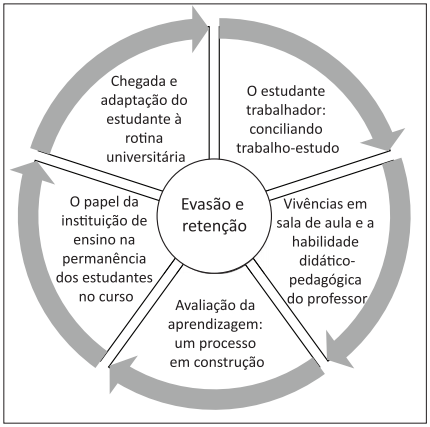
\includegraphics[width=0.6\textwidth]{./dados/figuras/proposta/evasao-retencao}
    \fonte{\citeonline{Lamers2017}}
    \label{fig:evasao-retencao}
\end{figure}

Assim, a possibilidade de antever o desempenho dos estudantes em disciplinas do ensino superior dentro de um espaço de tempo pode ser muito relevante, uma vez que pode-se tomar ações acerca dessa situação e se possível revertê-la.

Neste contexto, a mineração de dados pode ser empregada, com o uso de técnicas de aprendizado de máquina, a fim de realizar a detecção de padrões e definição de modelos que descrevam o comportamento da situação em discussão. Claramente, devido a natureza subjetiva do ambiente acadêmico, o número de variáveis que influenciam no desempenho dos alunos é muito grande, desta forma a acurácia associada à predição se torna muito dependente da qualidade, confiabilidade e volume dos dados disponíveis \cite{Caetano2016}.

A seguir é contextualizada a mineração de dados, bem como algumas de suas técnicas.

\section{MINERAÇÃO DE DADOS}
\label{sec:mineracaoDados}

Embora inicialmente direcionadas as áreas de negócios, as técnicas de mineração de dados se tornaram grandes ferramentas para a extração de conhecimento a partir de volumes de dados, e atualmente, diversos setores a utilizam para o reconhecimento de padrões e análise de dados \cite{Marques2015}.

\citeonline{Weis1999} definem a mineração de dados como a busca e extração de informações valiosas de grandes volumes de dados, com a cooperação entre o homem - que projeta os bancos de dados, descreve os problemas e define os objetivos desejados, e o computador - que verifica os dados buscando padrões que harmonizem com as metas definidas anteriormente. Muitos autores classificam a mineração de dados como a mistura dos campos de estudo da estatística, da inteligência artificial e dos bancos de dados \cite{Cortes2002}.

Para este trabalho foram empregadas técnicas de mineração de dados e aprendizado de máquina como forma de extração de informação e predição dos volumes de dados acadêmicos. A seguir são apresentadas as técnicas de mineração de dados utilizadas neste trabalho.

\subsection{Ferramentas Estatísticas}
    
A primeira técnica consiste das ferramentas estatísticas, utilizadas para efetuar análises simples do conjunto de dados a ser minerado. Muitas vezes com estas ferramentas é possível extrair informações relevantes sobre a distribuição dos conjuntos de dados. Alguns exemplos destas ferramentas são a média aritmética, valores mínimos e máximos, desvio padrão e a distribuição percentual dos dados.

Com estas informações é possível construir gráficos e outras ferramentas visuais que possibilitam uma análise inicial dos dados \cite{Adriaans1996}.

\subsection{Regressão Linear}
A regressão linear é uma técnica de predição numérica, e tem como objetivo estimar valores futuros para uma variável contínua, tentando encontrar uma relação com comportamento linear entre as variáveis preditoras.
Ou seja, onde é possível criar um modelo no qual o valor de uma variável \textit{y} pode ser descrita como uma função linear de uma variável \textit{x}.
Para esta técnica as variáveis preditoras são os atributos do conjunto de dados e usualmente é utilizada a abordagem dos mínimos quadrados para otimizar a função, minimizando a soma dos quadrados das diferenças entre o valor estimado e os dados reais \cite{Camilo2009}.
    
A \autoref{fig:regressao-linear} apresenta um exemplo de regressão linear, no qual é possível verificar uma relação entre as variáveis envolvidas por meio da linearidade entre elas.
Nesta verifica-se que o comportamento da variável 'Salários Mínimos' pode ser descrito aproximadamente como uma função linear da variável 'Anos de Experiências'. A linha contínua representa um exemplo de função linear que seria retornado por um modelo de regressão linear para este conjunto de dados.
    
\begin{figure}[!htb]
    \centering
    \caption{Exemplo de regressão linear, com a variável 'Salários Mínimos' em função da variável 'Anos de Experiências'}
    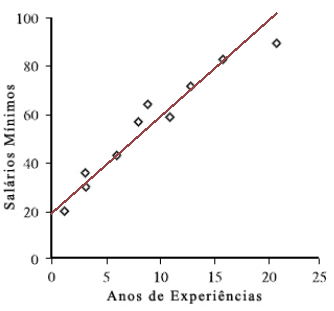
\includegraphics[width=0.5\textwidth]{./dados/figuras/proposta/regressao-linear2}
    \fonte{\citeonline{Camilo2009}}
        \label{fig:regressao-linear}(Adaptado)
    \end{figure}

\subsection{Arvore de Decisão}

A árvore de decisão é um método simples de aprendizado de máquina construído por um processo chamado de indução, que visa dividir os dados em subconjuntos de forma a entender as segmentações criadas para cada atributo, ou \textit{feature}, do modelo. 

Ela funciona como um fluxograma no formato de árvore, onde cada nó não folha apresenta um teste realizado sobre um valor, as ligações entre os nós possuem os valores possíveis para o teste efetuado, e os nós folha indicam a classe ao qual o registro foi determinado como pertencente.

Apesar da simplicidade do método, a árvore de decisão apresenta acurácia semelhante a de métodos mais complexos, porém demanda de uma análise detalhada dos dados para garantir que bons resultados sejam obtidos  \cite{Camilo2009}.

A \autoref{fig:arvore-decisao} apresenta um exemplo simplificado de árvore de decisão, onde é classificado a partir do atributo idade de uma determinada amostra a classe ao qual esta pertence. Os retângulos representam as regras ou testes, e as possíveis classes são representadas pelas elipses.

\begin{figure}[!htb]
    \centering
    \caption{Exemplo simplificado de árvore de decisão, com a classificação de faixa etária por meio da idade}
    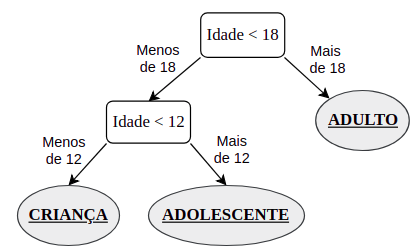
\includegraphics[width=0.6\textwidth]{./dados/figuras/proposta/arvore-decisao}
    \fonte{Autoria própria}
    \label{fig:arvore-decisao}
\end{figure}
    
\subsection{\textit{Random Forest}}
\label{ssec:randomForest}

O \textit{Random Forest} é uma técnica de aprendizado de máquina utilizada tanto para realizar regressões quanto classificações que utiliza múltiplas árvores de decisão para realizar suas predições.

Ela é considerada uma técnica do tipo \textit{bootstrap aggregation}, comumente chamado de \textit{bagging}. No \textit{bagging} algoritmos mais simples são treinados diversas vezes de forma independente utilizando diferentes subconjuntos de dados, gerados por meio de re-amostragem com reposição em um conjunto de treino inicial.

No caso do \textit{Random Forest}, múltiplas árvores de decisão são treinadas independentemente, tomando como base subconjuntos de treinamento formados a partir dos dados de treinamento inicial. 
E o resultado final do algoritmo é definido com base na agregação dos resultados obtidos para cada uma das árvores de decisão \cite{Liaw2002}.

Para classificação é comum o uso da maioria dos votos como estratégia para a definição da classe a ser retornada como resultado. Já para regressão são utilizadas ferramentas estatísticas, como a média aritmética dos resultados retornados por cada árvore de decisão.

A figura \ref{fig:random-forest} apresenta um exemplo simplificado de uma \textit{random forest} de classificação, nela são treinadas quatro árvores de decisão e o resultado da predição é determinado com base na classe que recebe a maioria dos votos, neste caso a classe C.

 \begin{figure}[!htb]
    \centering
    \caption{Exemplo simplificado de \textit{random forest} utilizada para classificação}
    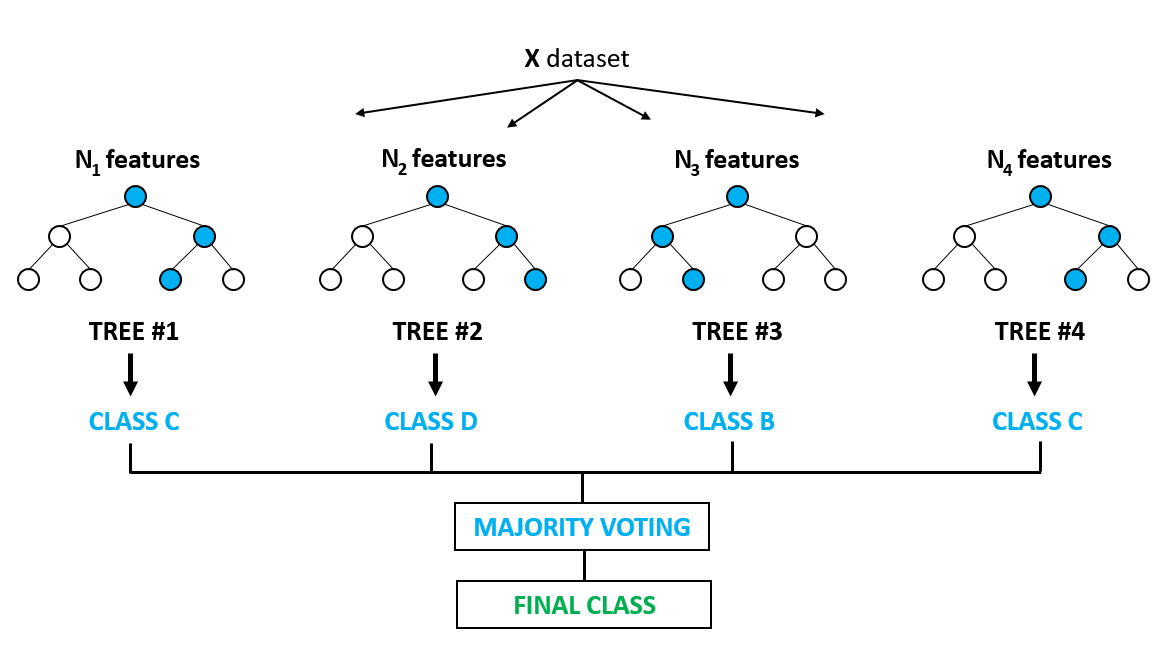
\includegraphics[width=0.8\textwidth]{./dados/figuras/random-forest}
    \fonte{Abilash R. (2018)}
    \label{fig:random-forest}
\end{figure}

\subsection{\textit{Gradient Boosting}}
\label{ssec:gradientBoosting}

Paralelo ao \textit{bagging}, apresentado anteriormente ao descrever o algoritmo \textit{Random Forest}, tem-se os algoritmos do tipo \textit{boosting}.

O princípio dos algoritmos de \textit{boosting} consiste da combinação do resultado de diversos classificadores ou regressores não tão eficientes, a fim de obter um algoritmo final com melhor acurácia. 
Diferente das técnicas de \textit{bagging}, que treinam modelos de forma independente, o \textit{Boosting} treina modelos com base no resultado e no erro de modelos anteriores, encadeando-os. Usualmente os algoritmos de \textit{boosting} utilizam árvores de decisão como algoritmo interno, mas não se limitam a elas \cite{Geron2017}.

Tendo as técnicas de mineração de dados delimitadas, foi-se então definido um modelo metodológico a ser seguido durante o desenvolvimento do trabalho.
A seguir será apresentado o CRISP-DM, modelo utilizado para demarcar as tarefas de um projeto de mineração de dados.

\section{CRISP-DM}
\label{ssec:crisp}
 
O CRISP-DM (\textit{Cross-Industry Standard Process for Data Mining}) é um modelo de processo amplamente utilizado para descrever as etapas da mineração de dados. Um exemplo da aplicação do método é apresentado por \citeonline{Castro2018}, no qual o CRISP-DM é aplicado à um cenário onde é realizado um processo de Busca de Conhecimento em Banco de Dados\footnote{Conhecido também como KDD (\textit{knowledge-discovery in databases}), é o processo de extração de informações valiosas implícitas em bases de dados.} visando a evasão no ensino superior.

O CRISP-DM é composto por seis etapas, que descrevem a sequência de fases para o desenvolvimento de um projeto de mineração de dados. Estas são apresentadas na \autoref{fig:crisp-dm} e são detalhadas a seguir \cite{Chapman2000, Shearer2000}.

\begin{figure}[!htb]
    \centering
    \caption{Método CRISP-DM de modelo de processo para mineração de dados}
    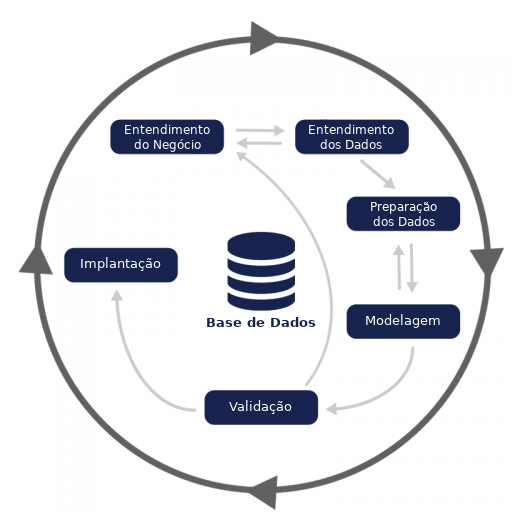
\includegraphics[width=0.6\textwidth]{./dados/figuras/proposta/crisp-dm}
    \fonte{\citeonline{Chapman2000}}
    \label{fig:crisp-dm}
\end{figure}

\subsection{Entendimento do Negócio}

Permite compreender os objetivos do projeto considerando uma perspectiva do negócio, auxiliando na definição do problema de mineração de dados. 
É importante posteriormente para compreender os dados que serão analisados e quais os tipos de valores que se deseja extrair deles.

Pode ser resumido nas seguintes subetapas: definição dos objetivos do negócio, avaliação da situação, definição dos objetivos de mineração de dados e construção do plano de projeto.

\subsection{Entendimento dos Dados}

Esta fase consiste basicamente das seguintes subetapas: coleta inicial dos dados, descrição dos dados, análise dos dados e verificação da qualidade dos dados.
Esta sequência de passos é efetuada de forma que, após a coleta inicial dos dados, objetiva-se desenvolver uma certa familiaridade com os dados, descrevendo-os, para assim identificar problemas de qualidade e subconjuntos de dados que possivelmente contenham informações implícitas.

\subsection{Preparação dos Dados}
\label{sssec:preparacaoDados}

Consiste do tratamento dos dados inicialmente coletados a fim de construir o conjunto final de dados que será utilizado para processamento e análise, e é subdividida em cinco etapas menores: seleção, limpeza, construção, integração e formatação dos dados.

Esta fase se dá inicialmente com a seleção dos dados que serão utilizados para a análise, verificando a sua relevância para os objetivos da mineração de dados, bem como a qualidade e as limitações técnicas quanto ao volume e tipos de dados. 

Após, tem-se a limpeza dos dados, que é responsável por remover dados ruidosos e sem valor para a análise, evitando assim ambiguidades e anomalias nos resultados. 
Nela é feita a conversão de dados que possam estar em um formato não adequado e a remoção de caracteres inválidos, podendo também ser efetuada uma normalização dos dados para ajustá-los à determinadas situações.
Remete a subfase do Entendimento dos Dados, que se refere a verificação da qualidade dos dados. 

Em seguida, na construção dos dados, há a transformação de certos atributos coletados em atributos projetados para facilitar a etapa de processamento, reduzindo em certos casos a quantidade necessária de atributos, como por exemplo ao transformar os atributos \textit{comprimento} e \textit{largura} em somente um atributo \textit{área}. 

Também é importante a integração dos conjuntos de dados coletados relacionando-os para a criação de novos registros, por exemplo quando dois conjuntos de dados possuem valores que podem ser relacionados para gerar dados mais concisos, mas estão fragmentados. 

Por fim tem-se a formatação dos dados, que redesenha o conjunto de dados a fim de permitir sua manipulação por algoritmos e ferramentas específicas.

\subsection{Modelagem}

Nesta etapa do processo são selecionadas técnicas de modelagem de acordo com o problema a ser resolvido. 
Em seguida são gerados testes empíricos para validar a aplicabilidade do modelo, por exemplo a classificação, abordagem supervisionada de aprendizado de máquina utilizada em mineração de dados, utiliza-se taxas de erro entre conjuntos de dados de treinamento e conjuntos de dados de teste para medir sua acurácia. Desta forma verifica-se se o modelo pode prever dados históricos com eficiência, para então utilizá-lo para predizer dados futuros. 

Então o modelo é gerado sobre o conjunto de dados preparados previamente e por fim é realizada a validação do modelo, avaliando a aplicação.

\subsection{Validação}

Nesta fase são avaliados os resultados apresentados pelo modelo, revisando a construção deste se necessário. Valida-se os resultados tomando em conta os objetivos do negócio definidos anteriormente, verificando se todos foram abordados de forma adequada ou se devem ser realizados ajustes nas etapas iniciais do processo. 

Por fim deve-se decidir como utilizar os resultados obtidos com a mineração de dados, caso estes sejam considerados satisfatórios e respondam ao problema de mineração de dados previamente definido.

\subsection{Implementação}

A implementação é a última etapa do CRISP-DM, mas isto não significa que o projeto é finalizado quando atinge esta etapa. 
Como apresentado na \autoref{fig:crisp-dm}, no qual o círculo com as setas mais externas representa a natureza cíclica da mineração de dados, onde se mantém em constante revisão e atualização.

Nesta fase as informações geradas a partir do processamento dos dados são organizadas e apresentadas ao usuário final (e.g. gerentes, analistas, clientes) por meio de gráficos e outras ferramentas de visualização de dados, a fim de auxiliar na análise e assim, nas suas tomadas de decisões.

\section{VISUALIZAÇÃO DE DADOS}

A visualização de dados descreve técnicas que objetiva-se a auxiliar na compreensão e extração de significado de dados utilizando contextos visuais.

Em um conjunto de dados podem haver informações importantes ocultas que podem auxiliar nas tomadas de decisão e a promover negócios.
Mas o desafio é que nem sempre é possível tirar conclusões apenas analisando números brutos.
Quando se analisa os dados apresentados em um formato visual, surgem padrões, conexões e outras descobertas que, de outro modo, não seriam percebidos \cite{Microsoft2018}.

Segundo \citeonline{Cortes2002}, a visualização de dados é extremamente útil como técnica de descobrimento de padrões, e embora possa parecer uma técnica não tão sofisticada, permite mensurar a qualidade inicial dos dados e identificar onde os padrões podem ser extraídos. 

Quando esta é utilizada em processos mais avançados de mineração de dados é possível a criação de gráficos tri-dimensionais interativos e gráficos de segmentação de bancos de dados em forma hierárquica, como uma árvore.

\section{TRABALHOS RELACIONADOS}
\label{sec:trabalhosRelacionados}

A seguir são apresentados trabalhos relacionados que possuem propostas com características semelhantes à deste trabalho.

Em seu trabalho, \citeonline{CorneliusJunior2015} apresenta um estudo sobre a evasão no ensino superior e a aplicação de técnicas de mineração de dados na tentativa de descobrir um perfil dos alunos com tendências evasivas e os padrões associados a essas tendências. 
O autor aplica as técnicas de classificação e associação utilizando a ferramenta de mineração de dados \textit{WEKA}, com base em um conjunto de dados cedidos pela Universidade de Santa Cruz do Sul. 
Neste contexto foram constatados que os fatores que mais influenciaram para a evasão de cursos foram o total de disciplinas cursadas e o status final das disciplinas do primeiro semestre acadêmico. 

\citeonline{Ramos2011} descrevem em seu trabalho uma pesquisa realizada com o objetivo de identificar determinantes para as questões de retenção e evasão no curso de Nutrição da UFRGS. 
Os autores utilizaram diversas abordagens para atingir o maior número de discentes, elaborando questionários eletrônicos para que fosse possível atingir tanto alunos em curso quanto alunos evadidos, e realizando entrevistas com alunos regulares e em situação de retenção. 
Com a conclusão do trabalho os autores explicitam a necessidade de criação de mecanismos de acompanhamento de alunos para a prevenção da retenção e evasão discente, bem como o desenvolvimento de competências relacionadas ao empreendedorismo, como forma de motivação para os alunos.

O trabalho de \citeonline{Marques2015} apresenta um projeto de pesquisa em andamento na área de mineração de dados educacionais, cujo objetivo é a predição do desempenho de estudantes universitários em ambientes convencionais de ensino. 
No trabalho os autores afirmam, que devido ao número elevado e a natureza não linear das variáveis que determinam o desempenho dos estudantes, a previsão pode nem sempre ser satisfatória e os resultados não serem suficientemente bons para tomadas de decisões que ajudem a corrigir os problemas do tema. 
Mas ainda se faz necessária a produção de trabalhos deste cunho, devido a possibilidade de antever, mesmo com certa margem de erro e de tempo, o comportamento de um aluno que se enquadra em um determinado perfil de desempenho, e então motivar o docente responsável pela disciplina a utilizar recursos pedagógicos que busquem recuperar o aluno ainda no tempo regular das aulas da disciplina.

Em um trabalho posterior, \citeonline{Caetano2016} apresenta uma aplicação de técnicas de aprendizado de máquina e mineração de dados com o foco na predição do desempenho acadêmico de alunos. 
Para isto a autora utilizou também o ambiente \textit{WEKA}, empregando três diferentes algoritmos de aprendizado de máquina: o \textit{Naive Bayes}, \textit{Nearest Neighbor} e o J48, versão do WEKA do algoritmo de árvore de decisões C4.5. 
O resultado do seu trabalho mostrou que foi possível prever o desempenho de estudantes com precisão de aproximadamente 70\% utilizando somente informações iniciais e 90\% caso seja utilizado um conjunto de atributos completo ou somente com os atributos mais impactantes para o treinamento do modelo.
Para este trabalho foram utilizados dados demográficos, como sexo, idade e estado civil, e dados associados ao desempenho parcial dos alunos, como notas dos trabalhos entregues durante o periodo letivo.

\citeonline{Rigo2015} apresentam em seu trabalho uma análise de melhorias possíveis na aplicação de mineração de dados educacionais, para que estes possam ser efetivamente utilizados para a detecção de padrões comportamentais relacionados à evasão escolar. 
Os autores salientam a necessidade de mapear os fatores associados ao fenômeno, bem como a necessidade de implantação de soluções interativas, que permitam o acesso dinâmico aos resultados e possibilite o diagnóstico precoce e a realização de ações pedagógicas relevantes para combater à evasão no ensino. 

O modelo proposto por \citeonline{Tinto1987} e posteriormente discutido por \citeonline{Andriola2006} propõe que as características demográficas, como o nível socioeconômico e os conhecimentos adquiridos previamente por meio de educação formal e informal, influenciam na integração do discente com o novo ambiente universitário, e a condição social do discente, como a idade, gênero, habilidades pessoais e expectativas de desenvolvimento pessoal, está fortemente associada com a motivação para o desempenho acadêmico e o seu reconhecimento.

\citeonline{Babosa2017} exploram em seu trabalho aspectos da mineração de dados como recurso tecnológico para investigações em um Ambiente Virtual de Aprendizagem (AVA). 
Com os resultados obtidos os autores indicam que a mineração de dados permite acesso a informações sobre o processo educativo, tais como aproveitamento, desempenho e a predição dos resultados finais, identificando relações entre dados que podem produzir novos conhecimentos. 
Isto permite refletir sobre os métodos de ensino empregados e então tomar decisões para a melhoria do desempenho acadêmico.